%% Простая презентация с примером включения программного кода и
%% пошаговых спецэффектов
\documentclass{beamer}
\usepackage{fontspec}
\usepackage{xunicode}
\usepackage{xltxtra}
\usepackage{xecyr}
\usepackage{hyperref}
\setmainfont[Mapping=tex-text]{DejaVu Serif}
\setsansfont[Mapping=tex-text]{DejaVu Sans}
\setmonofont[Mapping=tex-text]{DejaVu Sans Mono}
\usepackage{polyglossia}
\setdefaultlanguage{russian}
\usepackage{graphicx}

\begin{document}
\title{Реализация библиотеки для потоковой обработки .xlsx файлов}
%%\subtitle{предварительные результаты}
\author{Свитков Сергей\\{\footnotesize\textcolor{gray}{группа 344\\научный руководитель Ю.В. Литвинов\\консультант М.В. Заведеев}}}
\institute{СПбГУ\\кафедра системного программирования}
\frame{\titlepage}

\begin{frame}\frametitle{Введение}
\begin{itemize}
    \item Веб-приложения в сфере биллинга, телекоммуникаций
    \item Различные отчеты, статистика
    \item Формат .xlsx
    \item Потоковая обработка для экономии памяти
\end{itemize}
\end{frame}

\begin{frame}\frametitle{Существующие решения}
\begin{itemize}
    \item Apache POI
    \begin{itemize}
        \item До версии 3.8 --- только работа in-memory
        \item Начиная с 3.8 --- Stream-API для записи, Event-API для чтения
        \item Часть операций всё равно только in-memory
        \item Отсутствие полных и подробных примеров работы с Stream-API
    \end{itemize}
    \item SJXLSX
    \begin{itemize}
        \item Не поддерживается с 2015 года
    \end{itemize}
    \item Excel Streaming Reader
    \begin{itemize}
        \item Разработка коммьюнити
        \item Обертка над POI
    \end{itemize}
\end{itemize}
\end{frame}

\begin{frame}\frametitle{Постановка задачи}
\begin{itemize}
    \item Изучить существующие решения и формат xlsx
    \item Реализовать библиотеку для потоковой обработки xlsx файлов
    \item Опубликовать библиотеку в Maven
    \item Провести апробацию
    \item Сравнить полученную реализацию с существующими
\end{itemize}
\end{frame}

\begin{frame}\frametitle{XLSX}
\begin{itemize}
    \item zip-архив с xml файлами
    \item Структура:
    \begin{itemize}
        \item \texttt{Content\_Types}.xml --- типы контента в архиве и пути к ним
        \item \texttt{\_rels} --- зависимости между файлами внутри архива
        \item docProps --- метаданные: имя автора, дата создания, ...
        \item xl --- директория с основными файлами архива: workbook, страницы, стили, таблицы
    \end{itemize}
\end{itemize}
\end{frame}

\begin{frame}\frametitle{XLSX}
\begin{itemize}
    \item Workbook:
    \begin{itemize}
        \item Метаданные
        \item Ссылки на страницы с данными
    \end{itemize}
    \item Worksheet:
    \begin{itemize}
        \item Содержат данные
        \item 3 формата представления данных: Grid, Chart, Dialog 
    \end{itemize}
    \item Grid:
    \begin{itemize}
        \item Данные разбиты на ряды;
        \item Каждый ряд состоит из ячеек, в которых хранятся значения
        \item В каждой ячейке хранятся номер ряда и тип значения
    \end{itemize}
\end{itemize}
\end{frame}

\begin{frame}\frametitle{Реализация: подход}
\begin{itemize}
    \item Запись:
    \begin{itemize}
        \item Для каждой страницы создавать временный файл
        \item Хранить в RAM только один ряд (во время создания)
        \item После создания добавлять ряд во временный файл страницы
        \item После завершения формирования документа --- записывать данные из временных файлов в основной файл
        \item Для экономии дискового пространства сжимать временные файлы
    \end{itemize}
    \item Чтение:
    \begin{itemize}
        \item Использовать парсер POI
        \item Реализовать механизм передачи прочитанных данных пользовательскому обработчику
    \end{itemize}
\end{itemize}
\end{frame}

\begin{frame}
  \transwipe[direction=90]
  \frametitle{Архитектура решения}
  Упрощенная архитектура решения:
  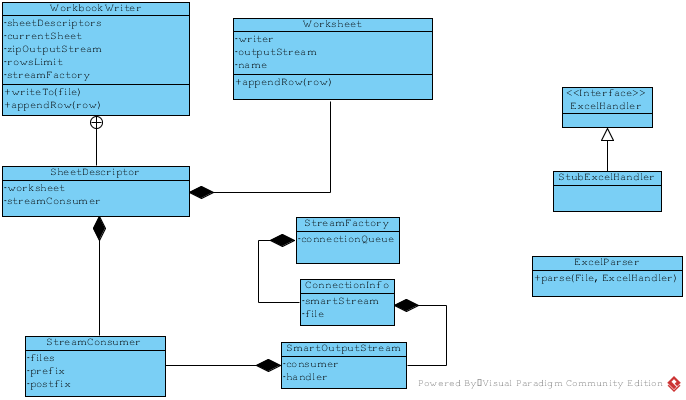
\includegraphics[width=\textwidth,height=\textheight,keepaspectratio]{arc.png}
\end{frame}

\begin{frame}\frametitle{Реализация}
\begin{itemize}
    \item Хранить in-memory только один ряд
    \item Уже созданные ряды записывать во временные файлы на диск
    \item Для экономии дискового пространства сжимать временные файлы
\end{itemize}
\end{frame}

\begin{frame}\frametitle{Текущие результаты}
\begin{itemize}
    \item Проведён анализ существующих решений и формата xlsx
    \item Разработана архитектура библиотеки
    \item Почти закончена реализация библиотеки
\end{itemize}
\end{frame}

%\lstset{language=java}
%\begin{frame}[fragile]\frametitle{Алгоритм}
%\begin{lstlisting}
%while (isWater()) {
%  row(boat);
%  if (crayfish) {
%    put(hand, river);
%  }
%}
%\end{lstlisting}
%\end{frame}

%\begin{frame}\frametitle{Результаты}
%\Large
%\begin{itemize}
%    \item Достигли
%    \begin{itemize}
%        \item того
%        \item сего
%    \end{itemize}
%    \item Получили
%    \item Обнаружили
%\end{itemize}
%\end{frame}
\end{document}